\section{Algorithmes de Dijkstra et A*}


\paragraph{Algorithmes de Dijkstra : }Edgser Wybe Dijkstra (EWD), physicien néerlandais reconverti à l'informatique en 1955, a proposé en 1959 un algorithme de recherche de chemin minimum dans un graphe dont la complexité est en $\mathcal{O}(n)$. 

\begin{figure}[htp]
  \centering
  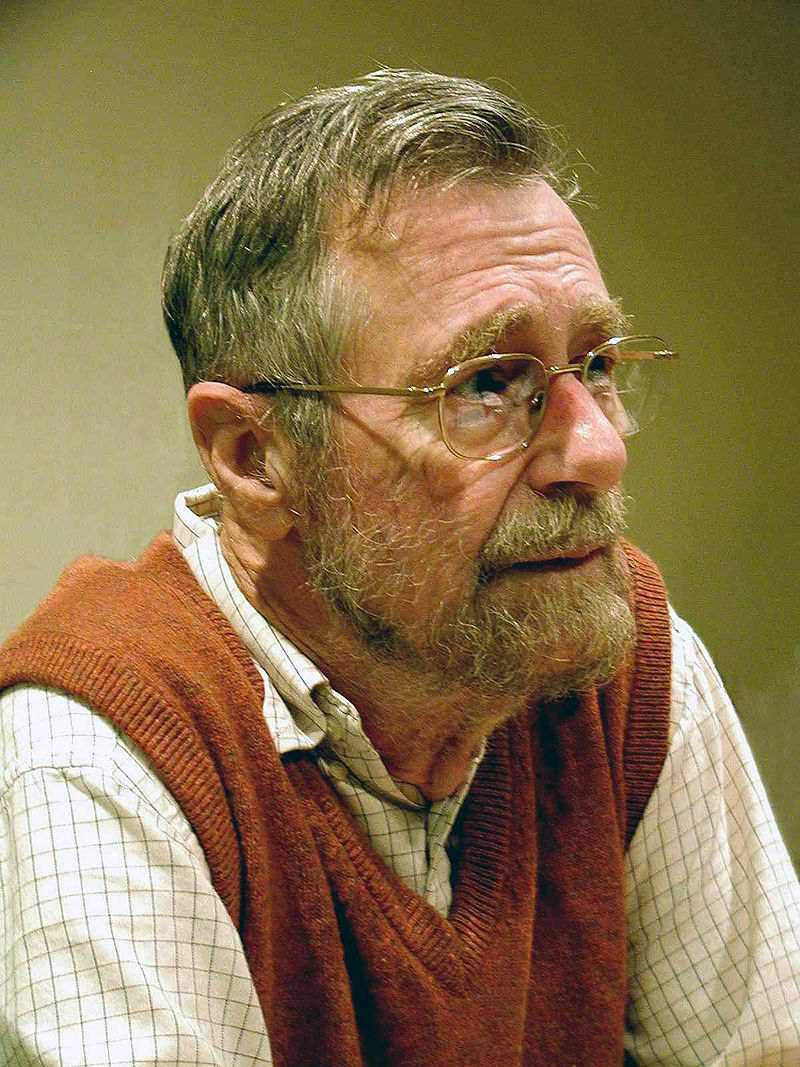
\includegraphics[width=4cm]{images/Edsger_Wybe_Dijkstra}
  \caption{Edgser Wybe Dijkstra (1930-2002)}
  \label{fig:une-autre-image}
\end{figure}

On doit à Dijkstra, qui avait la réputation d'avoir mauvais caractère et qui était notoirement allergique au ``GOTO'',
quelques citations\footnote{source : \url{https://fr.wikipedia.org/wiki/Edsger_Dijkstra}} telles que :


\begin{quote}
\textit{« Il est pratiquement impossible d'enseigner la bonne programmation aux étudiants 
qui ont eu une exposition antérieure au BASIC : comme programmeurs potentiels, 
ils sont mentalement mutilés, au-delà de tout espoir de régénération. »}
\end{quote}

\begin{quote}
\textit{« Le plus court chemin d'un graphe n'est jamais celui que l'on croit, 
il peut surgir de nulle part, et la plupart du temps, il n'existe pas. »}
\end{quote}

\begin{quote}
\textit{« La programmation par objets est une idée exceptionnellement mauvaise qui ne pouvait naître qu'en Californie. »}
\end{quote}


L'algorithme donne le plus court chemin de la source à \textit{tous les sommets} d'un graphe 
connexe pondéré (orienté ou non) dont le poids lié aux arêtes est positif ou nul.



%  \cite{Roque2012,Roque2012b,Roque2012c,Roque2012d}. 
 


\begin{figure}[htp]
  \centering
  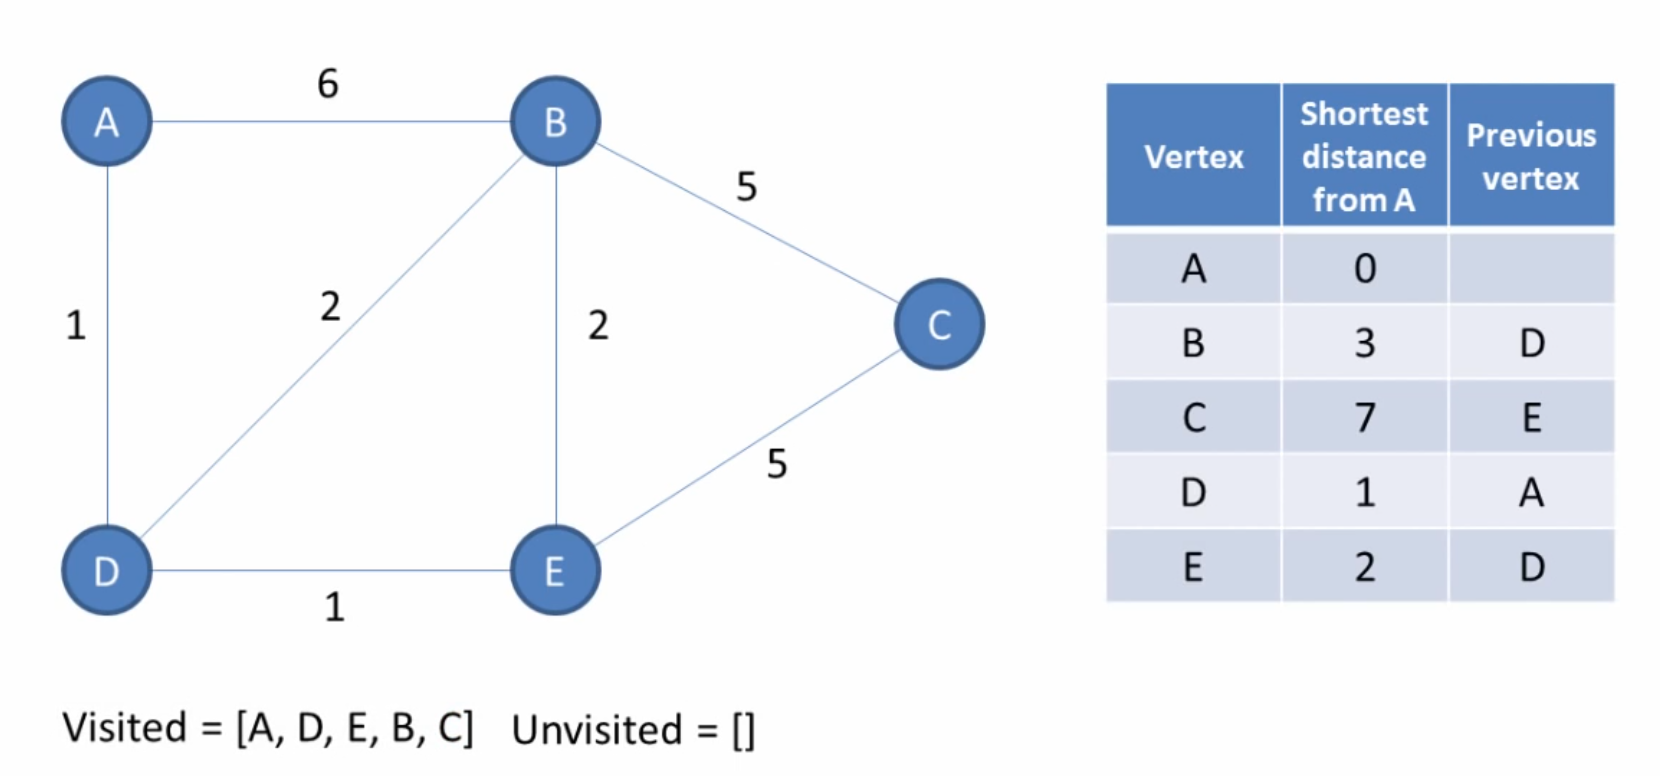
\includegraphics[width=15cm]{images/algo_dij}
  \caption{Exemple de calcul des plus courts chemins à partir du noeud A.}
  \label{fig:graph_dij}
\end{figure}

Sans entrer dans les détails d'implémentation que l'on trouve nombreux sur la toile et dans la littérature, l'algorithme de Dijkstra est 
un algorithme glouton qui utilise l'hypothèse qu'une décision prise sur la base
d'un critère d'optimalité locale conduira à un optimum global. Ainsi, à chaque itération, l'algorithme choisit, parmi les nœuds non traités, le nœud
du réseau dont la distance au nœud de départ est la plus faible. Ainsi, dans l'image \ref{fig:graph_dij}, on voit que le plus court chemin pour aller de A à C a un coût de 7. On détermine ensuite de proche en proche le chemin le plus court grâce à la mémorisation des nœuds précédents. Ici, C a pour ``previous vertex'' E, 
E -> D et D -> A. Le plus court chemin pour aller de A à C est donc ADEC. On utilise la même technique pour déterminer tous les chemins optimaux 
d'origine A. Mais on peut n'avoir besoin que du calcul du chemin entre 2 sommets. De plus, la myopie de l'algorithme limite forcément ses performances. D'où l'idée
d'utiliser une heuristique visant à guider les choix locaux. Ce qui nous amène à l'algorithme A* présenté brièvement dans la suite.

% \begin{figure}[htp]
%   \centering
%   \tikzstyle{block} = [draw, fill=blue!20, rectangle, minimum height=3em, minimum width=6em, text width=6em,text centered]
\begin{tikzpicture}[auto, node distance=3.5cm,>=latex']
\shorthandoff{:} % Evite le bug de compilation avec tikz
    % Longueurs et espacement
    \def\longabove{0.2cm}
    \def\espacement{4cm}

    % Définition des blocs
    \node [block, node distance=\espacement] (codeur) {Codeur};
    \node [block, right of=codeur, node distance=\espacement] (cbs) {CBS};
    \node [block, right of=cbs, node distance=\espacement] (modulateur) {Modulateur};
 
    % Définition des liens
    \draw [<-] (codeur) -- ++(-2,0) node[left] {$\{b_n\}$};
    \draw [->] (codeur) -- node[above=\longabove] {$\{d_n\}$} (cbs);
    \draw [->] (cbs) -- node[above=\longabove] {$\{c_k\}$} (modulateur);
    \draw [->] (modulateur) -- ++(2,0) node[right] {$s(t)$};
\end{tikzpicture}

%   \caption{Exemple de diagramme TikZ.}
%   \label{fig:une-image}
% \end{figure}
\paragraph{Algorithme A* : }

A* est l'algorithme qu'on utilise intuitivement pour se déplacer d'un endroit à un autre dans une ville
connaissant la direction à prendre. Grâce à cette information supplémentaire, A* va privilégier le nœud qui minimise 
la somme de la distance déjà parcourue et de la distance estimée restant à parcourir, qui peut être ici la distance à vol d'oiseau.


Cet algorithme a été proposé pour la première fois 
par Peter E. Hart, Nils John Nilsson et Bertram Raphael
en 1968. Il s'agit d'une extension de l'algorithme de Dijkstra et s'applique comme ce dernier
à des graphes munis d'une distance positive. En outre, A* ne teste pas tous les chemins ; il ne fournit donc
qu'un des meilleurs chemins. A* est cependant très performant dans le cas où le graphe comporte une faible densité de nœuds 
mais n'est pas ou peu efficace dans le cas de parcours de labyrinthes par exemple.


Il faut donc choisir, en fonction du problème, une heuristique $h$, c'est-à-dire ici une fonction qui estime la distance 
restante entre chaque nœud et l'arrivée, estimation par défaut qui ne doit jamais surestimer cette distance. 
La précision du résultat final dépendra de la précision de l'estimation.
On peut citer les heuristiques suivantes : la distance euclidienne (norme 2) ou à ``vol d'oiseau'' déjà citée 
et la distance de Manhattan (norme 1) qui, sur une grille, correspond à la somme des cases verticales et horizontales
qui sépare la position courante de l'arrivée. Les deux distances sont utilisables dans A* car elles sous-estiment
la distance à l'arrivée.

À chaque étape, l'algorithme calcule $g$, la distance déjà parcourue pour chaque nœud $n$ non visité puis
la valeur $f(n) = g(n) + h(n)$. Le nœud sélectionné est celui pour lequel $f$ est minimale. Lorsque l'heuristique est la fonction nulle, A* est équivalent à l'algorithme de Dijkstra.



\paragraph{Utilisation} L'application évidente de ces algorithmes dans le cadre du calcul parallèle est le transfert optimal de données d'un nœud \textit{A} vers un nœud \textit{B}. Cette application est d'ailleurs largement inspirée du domaine des réseaux de communication qui utilisent aussi la modélisation par graphes. On retrouve ainsi l'algorithme de Dijkstra dans le protocole de routage dynamique \textit{OSPF}.

On peut donc envisager optimiser un réseau de nœuds distribués en permettant l'ajout d'un nœud et sa prise en compte automatique par le réseau.

Quant à l'algorithme A*, il permettrait de déterminer un chemin point à point optimal utilisé ensuite par exemple pour créer une liaison par commutation de circuit intéressante si la taille des données qui doivent être échangées est importante.

There  are  many  different  heuristic  functions  used  for  the  grid  maps.  Some famous  heuristics  are 
Manhattan  distance,  diagonal  distance,  Euclidean  distance.  
We  are  using  the  Manhattan  distance  to  estimate  h(x)  because  it  works  better  on 
squared  grids. It  is  the  direct  distance  from  current  node  to  the  goal  node 
without considering obstacles in the path. In this way h(x) is giving us the lowest 
possible cos
t to reach the goal node


% \begin{table}[ht]
%   \begin{center}
%     \begin{tabular}{|c|c|c|c|c|}
%       \hline
%       & $h(t,\tau)$ & $S_{\OP{H}}^{(\alpha)} (f,\tau)$ & $L_{\OP{H}}^{(\alpha)} (\nu,t)$ & $H^{(\alpha)}(f,\nu)$ \\
%       \hline
%       LTI & $q(\tau)$ & $q(\tau) \delta(f)$ & $Q(\nu)$ & $Q(\nu) \delta(\nu-f)$ \\
%       \hline
%       LFI & $m(t) \delta(\tau)$ & $M(f) \delta(\tau)$ & $m(t)$ & $M(f)$\\
%       \hline
%       identité & $\delta(t)$ & $\delta(f)\delta(\tau)$ & $1$ & $\delta(\nu-f)$\\
%       \hline
%     \end{tabular}
%     \caption{Exemple de tableau.}
%     \label{tab:un-tableau}
%   \end{center}
% \end{table}


% \begin{figure}[htp]
%   \centering
%   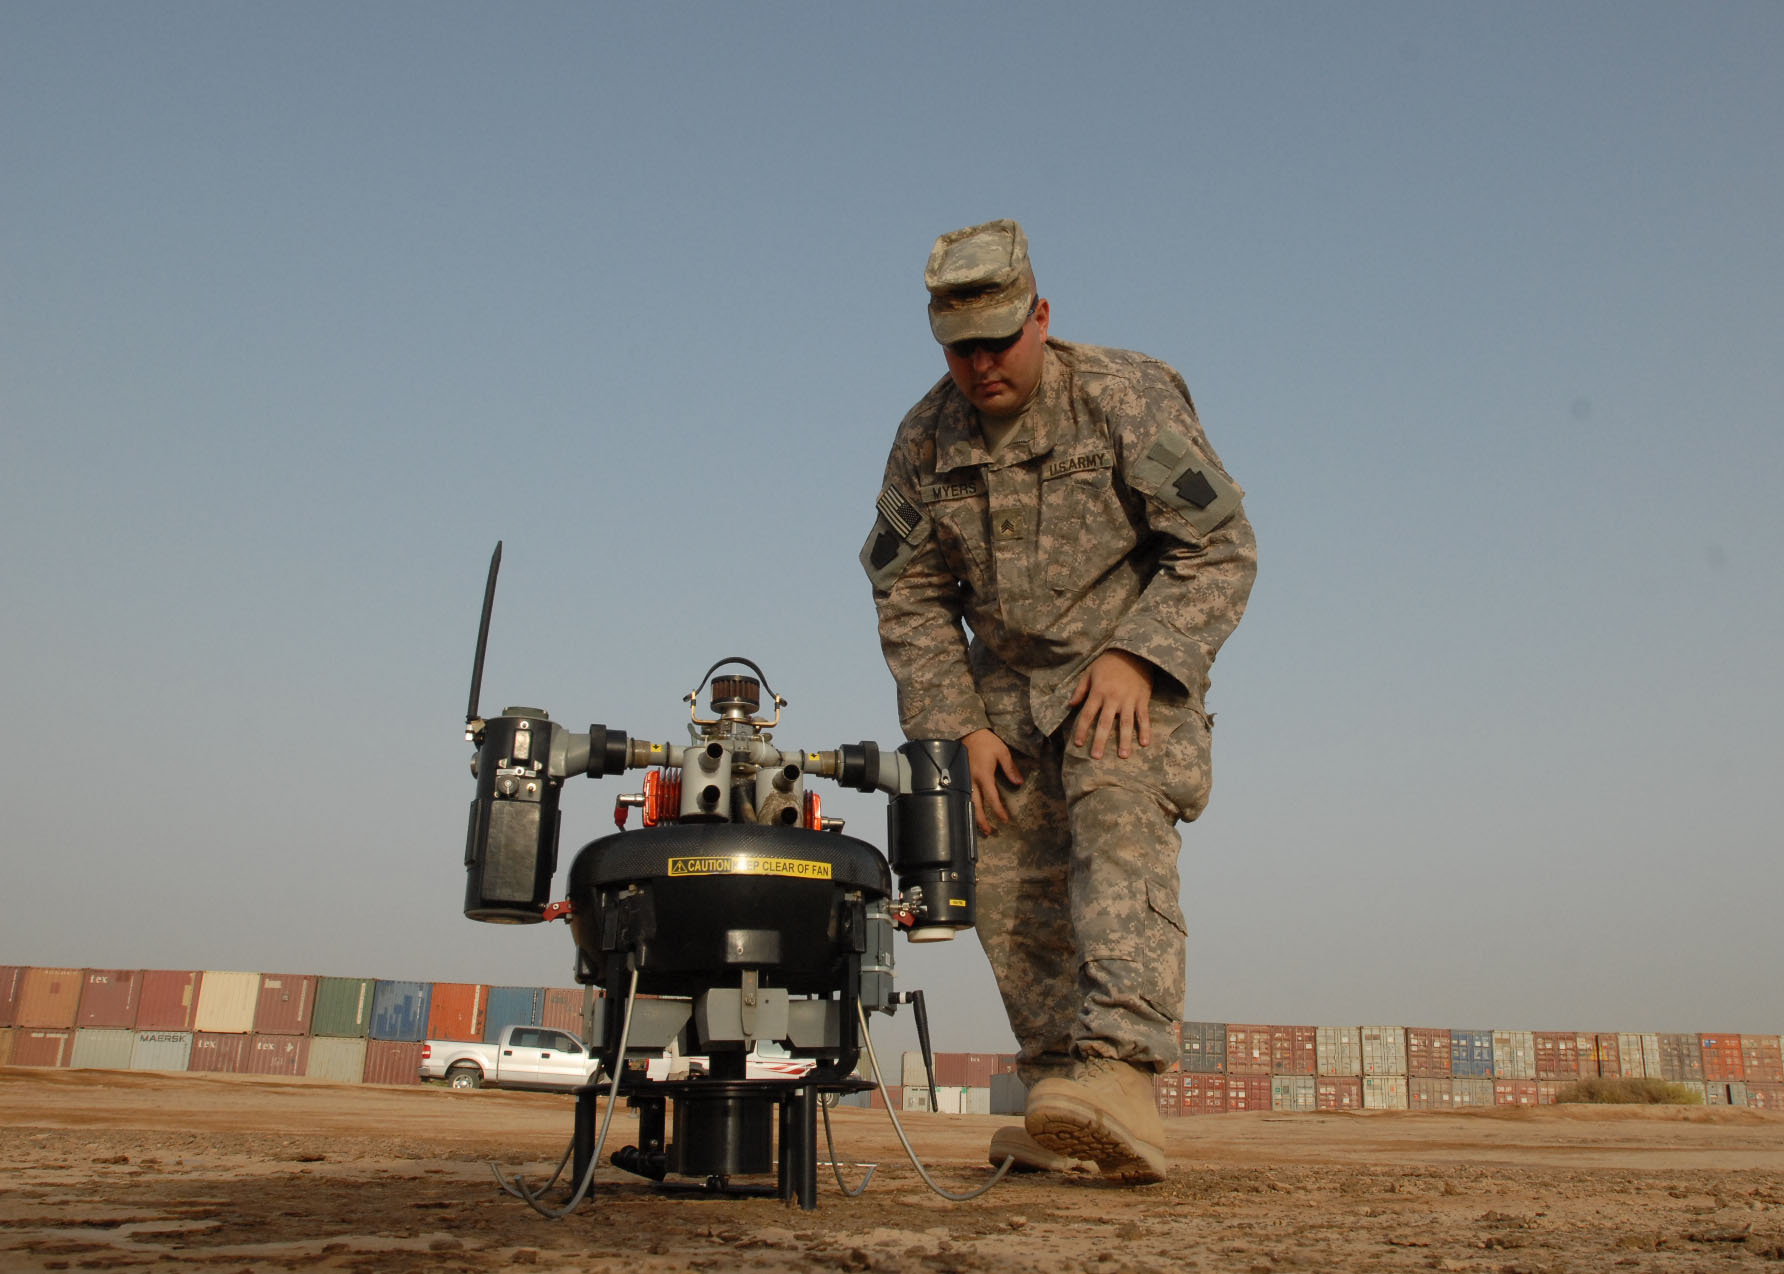
\includegraphics[width=4cm]{images/bitmap_image}
%   \caption{Exemple d'image au format JPG.}
%   \label{fig:une-autre-image}
% \end{figure}


%%% Local Variables: 
%%% mode: latex
%%% TeX-master: "isae-report-template"
%%% End: 